%%
%% Section 3
%%
%% 概要
%% 背景と目的
%% 方法と実現可能性
%% 期待される成果
%% 日本の独自性
%% 他のプロジェクトとの関係
%% 要求される装置とその仕様
%%
\section{日本が狙うサイエンス}\label{transients.s3}

本節では、SKAを用いた日本が主導するサイエンスについて述べる。
その中で、あるサイエンステーマを実現し成果を出すために、SKAに対してどのような装置要求をするべきか、あるいはSKAをどのように運用するべきかという戦略について言及する。
ただしSKAは既にそのデザインがおおよそ決まっているため、大幅な装置変更などは望めないことも考慮して、現状のデザインでどの程度のサイエンスが行えるか、ということについて主に述べる。

本研究は、宇宙における突発現象、変動現象を観測することによって、時間的に異なる宇宙の様相を捉え、そこから未解明の物理に迫ろうとするものであり、キャッチフレーズとして
\begin{center}
{\large \bf 「ダイナミックな宇宙を解き明かす時間領域の天文学」}
\end{center}
と題し、以下のようなサイエンスを提案する。
それらのサイエンスを日本で主導するため、SKAへ日本が参加することの重要性とSKAに対する要求に言及する。
\begin{itemize}
	\setlength{\leftskip}{3zw}
	\item [\ref{transients.s3.sn}] 系外超新星
	\item [\ref{transients.s3.snr}] 超新星残骸における粒子加速の現場、および星間物質と磁場の相互作用
	\item [\ref{transients.s3.grb}] 電波によるガンマ線バーストの即応追観測
	\item [\ref{transients.s3.magnetars}] マグネター磁気圏の解明
	\item [\ref{transients.s3.agn}] 死んだ電波銀河のシェルからの放射
	\item [\ref{transients.s3.gw}] 重力波--電波マルチメッセンジャー観測
	\item [\ref{transients.s3.frb.magnetism}] FRBの偏波の可能性と宇宙磁場	
	\item [\ref{transients.s3.unknowns}] 未知の突発天体の探査
	\item [\ref{transients.s3.requirements}] 突発天体研究のためのSKAへの要求
\end{itemize}

%%
%% Author: 前田啓一
%%
\subsection{系外超新星} \label{transients.s3.sn}

爆発直後の若い (一年程度以内の) 超新星における電波放射として支配的な機構は、超新星放出物質と星周物質の相互作用により発生する衝撃波と、そこで加速される相対論的電子からのシンクロトロン放射である \citep[e.g.,][]{1998ApJ...499..810C}。
これは現在の電波望遠鏡にとってはそれほど強い電波源ではなく、典型的な検出例では5~GHzにおいてピーク光度が$10^{27}~\text{erg}~\text{s}^{-1}~\text{Hz}^{-1}$ 程度の現象である \citep[e.g.,][]{2014arXiv1409.1827P}。
したがって、これまで電波観測されている数十例の系外超新星は、主に数十Mpc程度以内の距離で発生したものに限られており、非常にバイアスのかかった、限られたサンプルしか存在しない。

超新星の電波帯域における多様性は大きく、GRBに付随する極超新星 (SN 1998bwなど: \citealp{1998Natur.395..670G})、それと関連があると考えられている「相対論的」超新星 (SNe 2009bb, 2012ap: \citealp{2010Natur.463..513S})、あるいはIIn型超新星と呼ばれるタイプの一部 \citep[e.g.,][]{2012ApJ...755..110C} においては、その光度は$10^{29}~\text{erg}~\text{s}^{-1}~\text{Hz}^{-1}$ まで増光する。
タイムスケールも様々であり、5~GHz帯では典型的に数十日程度でピークを迎えるが、数年以上増光し続けるタイプのものも存在する。

観測されている電波放射の多様性は、超新星爆発により放出された物質の運動エネルギーおよび星周物質密度・分布の多様性を反映していると考えられ、電波放射の情報から星周物質密度などが導かれている \citep[e.g.,][]{2012ApJ...758...81M}。
一般に可視光観測からは星周物質の情報を直接導出することはできない。
超新星からの電波放射は、爆発直前の数十~数百年にわたる親星からの質量放出を反映するため、電波帯域における観測は、恒星進化論でも最大の謎の一つである大質量星の終末期の性質、超新星に至る直前の進化を知るためのユニークな手段である。
また、超新星残骸からの多波長放射により宇宙線加速機構の研究が進んでいるが、若い超新星においては衝撃波速度とダイナミクス、星周物質の密度が大きく異なる。
このため、宇宙線加速機構について超新星残骸を用いた研究とは別確度から切り込む新たな手段になると期待される。

SKAによる系外超新星研究は、主に可視で発見された超新星の即応追観測、SKA自体による電波サーベイの二つを並行して行うべきである。
現在世界中で様々な突発現象・超新星可視光サーベイが進行しており、SKAの時代には Large Synoptic Survey Telescope (LSST) の稼働が見込まれる。
日本においても木曽シュミット望遠鏡やすばる望遠鏡 Hyper Suprime-Cam (HSC) を用いた可視サーベイ計画が進展しつつある。
さらに、可視赤外大学間連携を通し可視・近赤外追観測の枠組みも整備され、恒星進化・超新星の理論研究を行うグループも多数存在しているなど、SKAの時代における即応追観測について存在感を発揮するための下地ができていると考えられる。
また、日本は歴史的に見ても電波観測におけるプレゼンスを発揮しており現在も大学間連携などを通し維持・発展しているのに加え、超新星電波放射の理論研究の下地もできつつある。
これらを総合し、可視--電波--理論を組み合わせた研究を進めるにあたり十分な下地ができていると言えるであろう。

\subsubsection{(1) 観測数の飛躍的増加によりもたらされる統計的理解}

超新星の性質の多様性を考えると、現在までの数十程度のサンプル数ではその全容を解明するためには全く不十分である。
SKAにおいては現在より少なくとも一桁良い観測精度を達成できるため、少なくとも数十倍の効率をもって、現在までの観測例とほぼ同等の質 (観測期間、S/N比など) のデータを取得できる。
たとえば年間一万個にのぼる発見が可能であるという見積もりも存在する \citep[e.g.,][]{2014arXiv1409.1827P}。
これにより、超新星の電波帯域における性質と可視光域における性質の関係が明らかになり、したがって爆発に至る進化 (電波) と超新星爆発の性質 (可視) の関係が明らかになるであろう。

\subsubsection{(2) まだ検出されていない電波放射の弱い超新星の研究}

従来の観測では、大半の超新星について電波放射は検出できていない。
つまり従来見つかっている超新星は、質量放出率の大きい系、爆発前に激しい質量放出をした系などが選択的に観測されたものであると考えられる。
また、既存の恒星進化理論では到底説明できないような、$0.1M_\odot~\text{year}^{-1}$以上の激しい質量放出が爆発直前に起こっている例も示唆されている \citep[e.g.,][]{2014ApJ...790L..16M}。
これらが特殊なのか一般的なのか明らかにするためには、より「弱い」電波放射をする超新星をとらえることが不可欠であり、これはSKAでなければ達成できない。

個々の問題についても、新たな電波放射検出が未解決問題解明のブレークスルーになり得る。
たとえば、Ia型超新星親星周辺の星周物質の有無・質量放出率は爆発に至る白色矮星の進化解明において最重要である \citep[e.g.,][]{2013FrPhy...8..116H}。
伴星が主系列星・巨星の場合 (single degenerate scenario: SD) には比較的濃い星周物質の存在が予測され、一方白色矮星二つの合体説 (double degenerate scenario: DD) からは希薄な周辺環境が予測される。
現在までの観測で、ごく近傍で発生した二つの超新星の星周密度について強い上限がついており、SD説に対し否定的な結果が得られている \citep{2014arXiv1409.1827P}。
同様の近傍Ia型超新星について弱い電波を実際に検出すること、さらに多くのサンプルについて強い上限値をつけることで、この議論に決着がつくであろう。
同様の議論はIa型超新星・重力崩壊型超新星の両方で見られる多様性の起源の解明のための大きな一歩となり得る。

\subsubsection{(3) 可視光では観測できない激しい星形成を起こしている銀河での超新星の検出と研究}

重力崩壊型超新星は大質量星の爆発であるため、その多くは激しい星形成を起こしている銀河で発生しているはずである。
しかし、luminous infrared galaxy (LIRG) や ultra luminous infrared galaxy (ULIRG)\footnote{光度が$10^{11}L_\odot$を超えるような赤外線で明るい銀河を LIRG とよび、$10^{12}L_\odot$を超えるものを ULIRG とよぶ。} といった星形成の激しい銀河は、一般的に可視光域では吸収が大きい銀河であり、そこで発生した超新星を可視光サーベイで発見することは困難である。
近年においては adaptive optics (AO) を用いた近赤外サーベイ、空間分解能の高い電波サーベイもなされているが、未だに数例の観測例が知られているだけである \citep[e.g.,][]{2007ApJ...659L...9M}。

超新星のイベントレートの測定は直接的な星形成率測定を与え、特に高赤方偏移に行くほど「隠された」星形成の割合は増えるため、イベントレートの解明は星形成史や初期質量関数の研究、超新星に至る恒星進化の研究にとって重要な要素である。
同時に、星形成の盛んな環境における超新星の性質が、これまで知られている超新星と同様であるかは自明ではない。
SKAにおける電波での広視野サーベイにより、このようなバイアスのかからない超新星のイベントレートや、様々な環境における超新星の性質・恒星進化、および初期質量関数の情報が得られるであろう。

\subsubsection{(4) 可視光観測とのシナジーによる近傍超新星の包括的研究}

これまでごく近傍の一握りの超新星について可視--電波の双方からの研究がなされているが、そのサンプル数の増大は重要である。
サンプル数が増えることによって、電波からわかる「親星の質量放出」と可視光からわかる「超新星の性質」との関係 (前述) や、様々な物理状況 (衝撃波速度、星周物質密度) における非熱的粒子加速 (後述) に加え、可視--電波観測のシナジーにより多くの新たな情報が得られる。
たとえば、電波による高い空間分解能の観測によって、ごく近傍の超新星については衝撃波伝搬の様子が直接撮像により求まる \citep[e.g.,][]{1995Sci...270.1475M}。また、爆発直後からの電波追観測により親星を衝撃波が突き抜けた直後 (ショックブレークアウト) の衝撃波速度を測定し、これから親星半径の情報を得ることができる \citep{2013ApJ...762L..24M}。
これらは最新の可視光観測手法と相補的であり、新たな研究分野を創出すると考えられる。

\subsubsection{(5) 強い衝撃波における相対論的電子加速機構、電子注入問題}

相対論的粒子加速機構は天体物理学における最重要未解明問題の一つである。
加速陽子の最大エネルギーが近年明らかになりつつあるが、それと同様に大きな問題として低エネルギー電子注入問題がある。
星周物質中を衝撃波が伝搬する若い超新星においては、物質密度したがって増幅磁場密度が大きいことがわかっており、GHz帯での観測によりMeV--GeV域の電子からの放射をとらえることができる \citep{2013ApJ...762L..24M}。
さまざまな星周物質密度をもつ異なる超新星の観測を包括的に行うことで、MeV--GeV域での加速電子スペクトルを得ることができるほか、ALMAなどによる高周波観測を組み合わせることで、個々の超新星における低エネルギー非熱的電子スペクトルを得ることができるであろう。
これは、電子注入問題を解明する上でのブレークスルーになり得る。
また、様々な環境で発生し様々な衝撃波物理状況を持つ様々な超新星を観測することにより、電子加速効率などを統計的に調べることが可能になり、これをもって粒子加速機構に必要・重要な条件を探ることができるであろう。




%%
%% Author: Shiu-Hang Lee, 長瀧重博
%%
\subsection{超新星残骸における粒子加速の現場、および星間物質と磁場の相互作用} \label{transients.s3.snr}

質量の大きな星々はその最期に超新星爆発とよばれる大爆発を起こすが、その後に何も残さない訳ではなく多様な物理現象がその後も続く。
多くの場合、超音速で膨張する星の残骸 (イジェクター) が様々な星間物質、あるいは星が「生前」放出した星風に衝突することによって衝撃波を形成する。
また衝撃波によってガスが高温に加熱され、陽子・電子などの帯電粒子が高エネルギーに加速されるなど非熱的な現象をも起こし、その結果電波・赤外線・可視光からX線・ガンマ線に至るまで多波長で見られる星雲状の天体を残す。
その何光年にも広がる天体は超新星残骸と呼ばれる。

超新星残骸は銀河の中の物理現象において様々な重要な役割を果たしていると考えられている。
例えば銀河系内宇宙線の生成、鉄など生命に不可欠な重元素の放出、星の形成、星間磁場の増幅などは、超新星残骸によって引き起こされるものである。
しかし、これまでに数多くの観測、理論モデリング、シミュレーションがなされてきたにもかかわらず、残骸中の物理は未だ完全には解明されておらず、実に複雑な天体であることが分かっている。
その問題が未解決であることの原因は、超新星残骸が年齢、親星の構造・組成、周囲の環境などの違いによって著しい多様性を示すこと、また既存の観測装置の性能限界とサンプル数の不足のためである。
そこでSKAのような、従来の観測装置の性能を遥かに超える次世代望遠鏡が、超新星残骸の理解のために非常に期待されている。
SKAを用いた科学や、そのためのSKAへの要求としては、以下のようなものが挙げられる。

\paragraph{(1) サンプル数の増大}
今まで発見された銀河系内の超新星残骸の数は僅か300に満たないが \citep{2014BASI...42...47G}、超新星の発生率を考えれば \cite[e.g.,][]{2006Natur.439...45D}、この数字は極端に少ない。
このことはつまり、まだ発見されていない超新星残骸が数多く残っているということであり、SKAの空間分解能と高感度があれば、これまでは暗すぎて観測できなかった残骸や、さらには系外天体の残骸についても多数発見出来ると考えられる。
また近傍銀河 (大マゼラン星雲、M33銀河など) の超新星残骸を探査することにより、若い残骸から古い残骸まで、超新星残骸の全体像を統計的に描けるようになる。
近傍銀河内の超新星残骸観測により、吸収のために観測しにくい天の川銀河内の残骸の真の分布も間接的に予想できるかもしれない。
更に他波長の観測装置 (Astro-H、CTA、ALMAなど) と緊密に連携し、多くの残骸を幅広いエネルギー域で調べることも可能となるだろう。

\paragraph{(2) 残骸の真の構造}
電波連続波で見る残骸はほとんどシェル状だが、その内部構造は複雑であり、特に衝撃波の周りではフィラメント状の構造が見つかる場合がある \citep[][]{1997ApJ...491..816R,2007A&A...471..537C,Reynolds2011}。
SKAを駆使することで、今まで感度不足のため見えなかった細かい構造を定量化し、モデリングを通して超新星残骸の真の三次元構造を明らかにできるだろう。
特にX線など他の波長との相関がより明確にわかるようになるため、超新星残骸中の非熱電子と磁場強度の分布を同時に解明できるようになり、無衡突衝撃波における粒子加速と磁場増幅の物理への理解を更に深めることにつながる。

\paragraph{(3) 粒子加速と磁場}
超新星残骸の電波連続波は主に加速された非熱電子によるシンクロトロン放射である。
SKAは広い波長帯をカバーしており、場所ごとの非熱電子のベキを精度よく測定できるようになると期待される。
また高感度で偏波観測を行えば、偏波率の小さい残骸に対しても、残骸内外の磁場の方向を推定することができる。
磁場の方向は衝撃波による粒子加速に大きく寄与するため \citep[][]{1996ApJ...473.1029E,2013AJ....145..104R,2014ApJ...783...91C}、SKAは高感度な偏波観測を行えるようデザインされなければならない。

\paragraph{(4) 星間物質との相互作用}
超新星残骸の多くは周りの星間物質 (星風、HI・分子雲など) と相互に強い影響を与え合い、明るい電波を放つ \citep{2000ApJ...538..203B,2012ApJ...746...82F}。
例えば、最近フェルミ衛星 \citep[e.g.,][]{2013Sci...339..807A} の観測によって、ガンマ線で明るくかつ爆発から1万年程度経った古い残骸は、そのほとんどが分子雲とぶつかっており、電波でも明るく観測されることがわかっている。
その放射機構・粒子加速機構はまだ謎のままだが、SKAによってこのような残骸を精度よくイメージングし、他の波長の観測データと組み合わせ、更にセルフコンシステントな理論モデル \cite[e.g.,][]{0004-637X-750-2-156} で解釈することにより、この謎は解明されると考えられる。
このとき他波長データとの比較のため、SKAはその資源を\Secref{transients.s2.wilkinson}で述べたVirtual Observatoryにささげることが重要である。



\input{transients/transients.s3.grb.tex}
%% Author: 榎戸 輝揚
\subsection{マグネター磁気圏の解明} \label{transients.s3.magnetars}
X線パルサーの中には、自転周期 2--12~s という遅い自転と、その自転周期が毎秒 $10^{-12}$--$10^{-10}~\text{s}$で遅くなるという極めて早い減速率を示し、そこから推定される磁場の強さが $10^{14}$--$10^{15}~\text{G}$ にも達するものが報告されている \citep{2008A&ARv..15..225M}。
さらに、観測されるX線光度が中性子星の自転では説明できないこともあり、それらのパルサーは内部に蓄えた磁場を解放して輝く超強磁場の天体と考えられるようになり、マグネターと呼ばれるようになった \citep{1995MNRAS.275..255T}。
このマグネターは、これまで銀河系内に 2000 個以上見つかってきた通常の回転駆動型パルサーとは異なる種族として、超新星爆発の機構や磁場の起源、強磁場の物理などの観点からも注目を集めている。

Swift衛星によって、突発的にX線で増光する銀河系内のマグネターも数多く見つかるようになり、すでに 30 個程度が知られている。
この発見をもたらした X 線アウトバースト現象では、$k_\text{B}T \sim 0.3~\text{keV}$ にピークをもつ星表面の熱的放射が増光するとともに、硬X線にピークをもつショートバーストを頻発し 100~keV 近くに向かって伸びる硬X線のべき放射も検出されるようになってきた \citep{2010ApJ...715..665E}。
こういった突発現象は通常の電波パルサーと異なるマグネターの特徴で、多波長でのフォローアップが急速に進展している。

通常の電波パルサーと異なり、定常的に明るく輝くマグネターでは、多くの場合電波のパルス放射が検出されていない。
たとえばGreen Bank 望遠鏡を用いた 1950~MHzの電波観測では、マグネター候補7天体で電波パルスは観測されなかった \citep{2012ApJ...744...97L}。
しかし一方で、X線アウトバーストを生じた際には電波が放射されるという例が報告されるようになってきた。
2003年に発見された XTE~J1810-197 \citep{2006Natur.442..892C} や2007年に突発増光した 1E~1547.0-5408 (PSR~J1550-5418; \citealt{2008ApJ...679..681C}) では、GHz 帯域でフラットなスペクトルを示し、100\% に近い直線偏光を示すなど、共通点をもった電波パルスが報告された。
さらに、電波観測によって最初に発見されたマグネター PSR~J1622-4950 \citep{2010ApJ...721L..33L}や、2013 年に銀河中心で見つかったマグネター SGR~1745-29 (PSR~J1745-2900; \citealt{2013ApJ...770L..23M}, \citealt{2014ApJ...780L...3S}) など、電波帯域でもマグネターの観測例が蓄積されつつある。

マグネターはX 線で卓越した放射を示すため、これまでは主に高エネルギー帯域の観測が主だったが、トランジェント型のマグネターの電波観測が新しい観測の窓とし
て開かれつつある。
また、定常的に明るい天体からも微弱な電波パルスが検出できるようになることも期待される。
従来、電波パルサーの多波長に渡るパルス研究がパルサー磁気圏の理解を進ませたように、SKA による電波観測を可視光やX線と組み合わせた多波長の突発現象観測が、マグネターの磁気圏の解明の伴になると期待できる。
%%
%% Author: 伊藤裕貴
%%
\subsection{死んだ電波銀河のシェルからの放射}\label{transients.s3.agn}
電波銀河の主な放射源は、AGNジェットによって形成される電波ローブと呼ばれる広がった構造である。
観測されている電波銀河のサイズは幅広く分布しており、kpc未満のものからMpcを超えるようなものまで存在している。
電波銀河の大きさは、主に年齢 (ジェットの中心核からの噴出が維持されている時間) によって決まり、小さいものは若く、大きいものは年老いていると考えられている。
したがって、小さい電波銀河はいずれ大きい電波銀河に成長するといった描像が広く受け入れられている。

しかしながら、単純に全ての電波銀河が10~kpcを超えるような大きさに成長できるのかはよく分かっていない。
というのも、理論的には 10~kpcに満たない小さくて若い電波銀河 (年齢$10^3$--$10^5$歳の電波銀河) の割合は全体の約 0.01\% と予測されるが、実際の観測では全体の約 10--30\% を占めており、年老いた銀河が予測より少ないためである \citep{Orienti01032010,2010MNRAS.408.2261K}。
この未解決問題について様々なシナリオが提唱されてきているが、一つの自然な解釈は、大多数の電波銀河が若い段階でジェット活動を停止もしくは休止し、成長が止まってしまい「死んでいる」とする解釈である。

このシナリオを検証するためには、死んだ電波銀河を観測でとらえる必要性があるが、ジェットの活動性を失った電波ローブは急激に暗くなってしまうため、従来の観測施設でとらえる事は困難であり、現状は候補天体が数例見つかっている程度である。
さらに最近の理論研究からは、ローブは暗くなるだけではなく放射帯域が10~MHz以下となってしまうため、SKA をもってしても、死んだ天体の電波ローブからの放射を検出する事は難しい事が示されている (Ito et al., 2015, submitted to ApJ)。
しかし電波ローブではなく、それを取り囲む周辺物質から構成される「シェル」は、ジェットの活動が休止した後も急激には減光しないため、SKAによってとらえられる事が期待できる (\Figref{fig:transients.s3.agn.fig1})。
したがって、電波銀河の進化トラック解明への道を切り開くためには、SKAを用いてシェルの観測を行うことが不可欠である。
さらにSKAによって、AGNジェットが周辺環境に与える影響 (AGNフィードバック) や、ジェットが駆動される条件などのサイエンスに関しても迫る事が期待される。
\begin{figure}
		\centering
		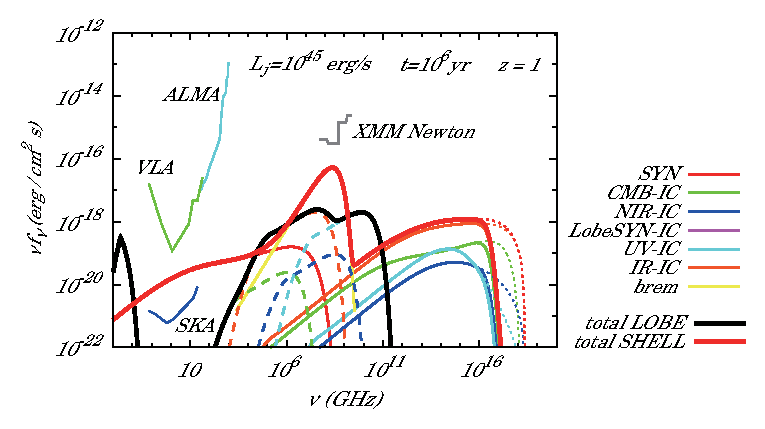
\includegraphics[width=0.8\textwidth]{transients/transients.s3.agn.fig1.eps}
		\caption{ジェットの放出が停止した (死んだ) 電波銀河に付随するローブ (黒実線) 及びシェル (赤実線) のスペクトル。
		電波銀河の年齢を$10^6$年、ジェットが活動を停止するまでの継続時間を$10^5$年と仮定し、また赤方偏移を$z=1$としている (Ito et al., 2015, submitted to ApJ)。}
		\label{fig:transients.s3.agn.fig1}
\end{figure}%

%% Author: 端山和大

\subsection{重力波--電波マルチメッセンジャー観測} \label{transients.s3.gw}
近年、オーストラリアのParkes電波望遠鏡によりFRBと呼ばれる継続時間数msの突発的な電波天体が相次いで観測され (\Secref{transients.s1.frb})、日本でも \Figref{fig:transients.s3.gw.nasu}の那須電波観測所によって、数分から数日といったFRBより長いタイムスケールの突発天体 (WJN電波トランジェント; \Secref{transients.s3.unknowns}) が観測されている。
こういった電波帯域における突発天体は未だ対応天体が発見されておらず、その起源の解明はこれからの電波天文学にとって重要なテーマの一つである。
\begin{figure}
	\centering
	\includegraphics[width=1\textwidth]{transients/transients.s3.gw.nasu.eps}
	\caption{那須電波観測所。口径 20~m の電波望遠鏡8基、30~mの電波望遠鏡1基をもつ。}
	\label{fig:transients.s3.gw.nasu}
\end{figure}%

こうした突発天体は、そのエネルギーとタイムスケールから、重力波を伴うような天体爆発現象である可能性が示唆されている。
FRBのモデルとしては、重力波天体として最有力候補の一つである中性子連星合体時に起きるシンクロトロン放射\citep{2013PASJ...65L..12T}があり、またWJNイベントのモデルとしては、中性子星連星合体後に起きる電波アフターグローモデルが考えられる \citep{2011Natur.478...82N}。
さらに連星合体の際は、\Secref{transients.s1.grb}で述べたようにshort GRBも付随することが予想される。
そこで重力波と電波を中心とした、「マルチメッセンジャー観測」と呼ばれる多粒子・多波長による連携観測により、天体現象の多角的理解を目指す観測体制の構築が重要になる \citep{2012IAUS..285..331H}。

FRBの本来のイベントレートはおよそ$2 \times 10^4~\text{Gpc}^{-3}~\text{yr}^{-1}$ と見積もられており、現在建設中の重力波望遠鏡が見通せる、地球から$200~\text{Mpc}$ 以内で起こりうるFRBは、年間$160$ 個程度と考えられる。
このイベントレートは現在見積もられている連星中性子星合体のイベントレートの誤差範囲内にある。
もしFRBの起源が重力波天体であり、かつすべて検出できるならば、2020年には年間$160$程度の重力波--FRB同時観測が行われ、統計的な議論もできるようになると考えられる。
こうした突発天体を捉えるためには広い視野で長期間観測して天球上を走査することが最も有効になる。
SKAで採用が検討されている Phased Array Feed (PAF) は $18~\text{deg}^2$ という広い視野を持ち、\skasur{1} プログラムでは1年間で$550$時間、走査領域にして$10,000~\text{deg}^2$をカバーすることが予定されており、非常に有望な重力波マルチメッセンジャー観測体制を担う望遠鏡である。
さらにSKAでAdvanced Instrumentation Program (AIP) となっているMid-frequency Aperture Array (MAA) は、$200~\sqdeg$という驚異的な広視野を持ち、その実装は電波天文学のみならず重力波天文学にとっても極めて重要である。

\subsection{FRBの偏波の可能性と宇宙磁場} \label{transients.s3.frb.magnetism}

今現在までに、FRBに有意な直線偏波は検出されていない\footnote{円偏波は1例観測された \citep{2015MNRAS.447..246P}。}。それがFRB現象に普遍的な現象なのか、または偶然なのか、その判断をするにはまだ発見数はあまりにも少ない。もしFRBに直線偏波が含まれるなら、ファラデー効果の分散測度 (DM) に加えてファラデー回転測度 (RM) も計測できる可能性がある。そうなった場合、密度重みつき視線平均磁場強度$\langle B_\parallel \rangle $をDMとRMの定義から
\begin{equation}
\langle B_\parallel \rangle =\frac{{\it RM}}{{\it DM}}
\end{equation}
という式で簡単に求めることができる。FRBが系外起源であるならば、この磁場強度の推定には銀河間磁場の情報を含む。電波銀河など系外偏波源を使ってRMを測る場合はDMは測らない (測れない) ため、このように単一観測から磁場強度まで推定できるのは画期的なことである。一つの視線だけでは系内と系外の寄与を切り分けるのは難しいかもしれないが、沢山の観測で統計を高めることで、銀経・銀緯に依存しないが赤方偏移に依存するような「超過成分」として銀河間磁場の寄与が議論できるかもしれない。SKAのサーベイ能力は、そのような統計的な議論をはじめて可能にするだろう。具体的で確実な調査の方法論を理論的に検討していくことも不可欠であるが、日本は銀河間磁場の調査で世界をリードしているので\citep{2014PASJ...66...65A,2014ApJ...790..123A}、日本のSKAサイエンスの特色の一つとできるだろう。FRBが銀河間磁場を探る新しい方法となるかもしれない。
\input{transients/transients.s3.unknowns.tex}
\input{transients/transients.s3.requirements.tex}
